\section{Model Predictive Control}
\label{sec:mpc}
Following the identification of the model done in section \ref{sec:trajectory_optimization}, an optimal control strategy was developed for the deployment of the zone heating by means of model predictive control (MPC). First, a primal optimal problem was developed for the MPC application which resulted in a significant decrease in energy consumption and therefore energy costs. Nevertheless, due to the constraint nature of primal optimal problems, the robustness of the control was a matter of concern. Due to this, a second approach following a lagrangian problem statement was developed. This allowed for the relaxation of the constraints, leading to a more robust control. The details pertaining both approaches are thoroughly explained in their corresponding subsections in the following.

\subsection{Primal MPC}
\label{subsec:primal_mpc}
As a first step, the calculated constants from section \ref{sec:trajectory_optimization} were used to develop the model. In order to ensure a proper MPC development, model state and control variables were determined. For this, the zone temperature $T_z$, ambient temperature $T_a$, solar radiation $\dot{Q}_{sun}$ and the heat input due to occupancy $\dot{Q}_g$ were taken as the system states $\boldsymbol{X}$. Since the goal of the MPC is the optimal deployment of the zone heating $\dot{Q}_{h}$, it was taken as the control variable $U$. The following code shows how these were expressed.

\begin{python}
    # constants
    N = len(time)  # number of samples
    delta_t = 3600  # s in 1 hour
    R = R_opt
    C = C_opt
    gA = gA_opt

    nx = 4  # number of states for system

    # Initializing optimization problem
    opti = Opti()

    X = opti.variable(nx, N + 1)  # states: Tz [K], Ta [K], Qsun [W/m2], Qg [W]. Multiple shooting

    U = opti.variable(N, 1)  # control variable: Qh [W]
\end{python}

Here, it can be seen that the state variable vector is initialized as a 4 by N+1 vector. This is since the transcription method used during this optimization is multiple shooting, which requires an additional state instance when compared to the control vector.\\

Moreover, the state vector was filled by means of a for-loop, following equation \ref{eq:finite_difference} and populating the rest of the states from the data collected in appendix \ref{appendix}.
\begin{python}
# Setting shooting constraints
for i in range(N - 1):
    opti.subject_to(X[0, i+1] == delta_t * ((X[2,i] * gA + U[i] + X[3,i])/C + (X[1,i] - X[0,i])/(R*C)) + X[0,i])
    opti.subject_to(X[1, i + 1] == temp[i + 1])
    opti.subject_to(X[2, i + 1] == Qsun[i + 1])
    opti.subject_to(X[3, i + 1] == Qg[i + 1])
\end{python}

Here, the first state is fully determined as a function of the control values, allowing for the optimization of its deployment. Additionally, the first instance for all states is purposefully skipped since the initial conditions are set at a later stage by means of the initial guess vector $\boldsymbol{X}_0$.\\

Next, the matter of constraints is considered. For this, first the physical limits for the radiator are stated by setting the control variables to be within 0 and 1000 W (its maximal heating output). Furthermore, the thermal comfort limits were placed for the zone temperature for instances on which someone is occupying the zone. This allows for the reduction of heating output during non-occupation times, leading to lower electrical costs. For this, a typical occupational time range was used on which there is one person inside the zone during the entire weekend and the zone is not occupied in the weekdays from 07:00 to 18:00.

\begin{python}
# setting bounded constraints (temp range for the zone whenever someone is home)
opti.subject_to(opti.bounded(293.15, X[0, 0:24], 298.15))  # weekend
opti.subject_to(opti.bounded(293.15, X[0, 144:], 298.15))  # weekend
for i in range(6):  # weekdays
   opti.subject_to(opti.bounded(293.15, X[0,0+24*(i+1):7+24*(i+1)], 298.15))
   opti.subject_to(opti.bounded(293.15, X[0,18+24*(i+1):24+24*(i+1)], 298.15))

# bounded constraints for max and min power output for the radiator
opti.subject_to(opti.bounded(0, U, 1000))
\end{python}

Next, initial conditions as well as the objective function were stated. Since the goal of the MPC is the reduction of energy consumption, the squared sum of the total heat deployed into the zone via the radiator $\sum \dot{Q}_{h}^2$ was declared as the cost function. The following snippet illustrates how both were introduced into CasADi.

\begin{python}
# setting initial conditions
opti.subject_to(X[:, 0] == x0)

# setting minimization equation
opti.minimize(sumsqr(U))

opti.set_value(x0, vertcat(293.15, temp[0], Qsun[0], Qg[0]))

opti.solver('ipopt')
sol = opti.solve()
\end{python}

The optimal control problem is then ready to be solved by means of the IPOPT solver. In order to provide more clarity, equations \ref{eq:mpc1} to \ref{eq:mpc2} summarize the above stated code in equation form.


\begin{equation}
{\text{minimize}} \hspace{1em} \sum_{i=1}^{N} \left(\dot{Q}_{h,i}\right)^2
\label{eq:mpc1}
\end{equation}
\begin{equation}
\text{subject to}  \hspace{1em} T_{z,i+1} - \Delta t \left( \frac{\dot{Q}_{h,i} + gA \cdot \dot{Q}_{sun, i} + \dot{Q}_{g,i}}{C_z} + \frac{T_{z,i}-T_{a,i}}{R_w \cdot C_z} \right) - T_{z,i} =0
\end{equation}
\vspace{-0.5em}
\begin{align}
\left[T_{z,0}, T_{a,0}, \dot{Q}_{sun,0}, \dot{Q}_{g,0}\right]^{\top}  - \boldsymbol{X}_0 &=  0 \\[0.5em]
T_{z,i} - 298.15 &\leq 0 \hspace{2em} \forall i \in \text{occupied}\\[0.5em]
293.15 - T_{z,i} &\leq 0 \hspace{2em} \forall i \in \text{occupied}\\[0.5em]
\dot{Q}_{h,i} - 1000 &\leq 0\\[0.5em]
-\dot{Q}_{h,i} &\leq 0
\label{eq:mpc2}
\end{align}

Lastly, the above stated MPC results in the temperature and heating deployment profiles seen in Figure \ref{fig:mpc_primal}.

\begin{figure}[H]
\centering
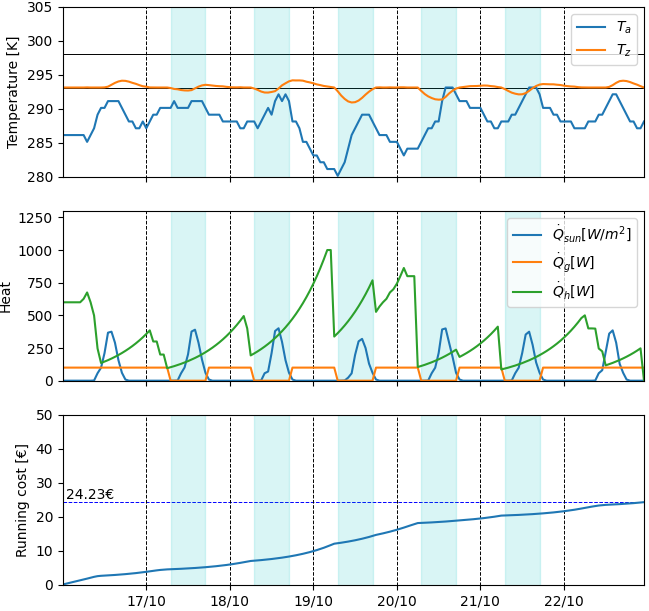
\includegraphics[scale=0.8]{images/mpc_primal.png}
\caption{MPC by means of a primal optimal problem for the zone heat deployment.}
\label{fig:mpc_primal}
\end{figure}

Immediately, when comparing Figures \ref{fig:mpc_primal} and \ref{fig:onoff_radiator} a decrease in weekly cost of about 30\% can be seen. Additionally, this cost reduction comes with a more stable temperature profile for the zone, ensuring thermal comfort at all occupant times. It can also be noted that the heat deployment is maintained well below the maximum power output for most days, helping towards the reduction of energy use.\\

While appreciating the benefits of the integrated MPC, the issue of robustness raises a large concern for the application of this system. This is due mainly to the strictness of the constraints for the zone temperature profile. By introducing the thermal comfort boundaries for the zone as a bounded constraint, we do not allow for considerations of exterior influences causing a drastic change in zone temperature and taking the zone outside of its comfort range (e.g. an open window, sudden rain, etc.). This effect is easily tested by varying the initial temperature for the zone since, at the first instance of the week, the thermal comfort constraint is valid. The following changes to the initial vector

\begin{python}
opti.set_value(x0, vertcat(253.15, temp[0], Qsun[0], Qg[0]))

opti.solver('ipopt')
sol = opti.solve()
\end{python}

quickly back the hypothesis since, by enforcing a temperature outside of the thermal comfort range, the solver is unable to return a solution and instead gives the error \texttt{return\_status is `Infeasible\_Problem\_Detected'}.\\

For this reason, it was decided that these constraints should be relaxed in order to increase the robustness of the system. This is done by means of a lagrangian problem statement, which is developed in the following subsection.

\newpage
\subsection{Lagrangian MPC}
\label{subsec:lagrangian_mpc}
Considering the robustness issues discussed in subsection \ref{subsec:primal_mpc}, a lagrangian approach was taken. For this, the same initial steps were taken as before. The distinction between both approaches is seen during the constraints setting portion of the code. When taking a lagrangian problem statement, the relaxed constraints are moved into the cost function alongside a weight factor for each constraint. Nevertheless, since some hard constraints (the maximum heating output for the radiator) are still necessary to maintain the physical limits of the system, not all constraints were introduced into the cost function. 

\begin{python}
    # setting minimization equation in lagrangian form
    mu1_val = 130
    mu2_val = 150

    # set the weights to a certain percentage for 'at work' hours
    mu1 = np.ones(N) * mu1_val * 0.8
    mu2 = np.ones(N) * mu2_val * 0.8

    # values for 0.8mu whenever no one is home, mu_val whenever someone is
    mu1[0:24] = mu1_val  # weekend
    mu1[144:] = mu1_val
    mu2[0:24] = mu2_val
    mu2[144:] = mu2_val
    for i in range(6):  # weekdays
        mu1[0 + 24 * (i + 1):7 + 24 * (i + 1)] = mu1_val
        mu2[0 + 24 * (i + 1):7 + 24 * (i + 1)] = mu2_val
        mu1[18 + 24 * (i + 1):24 + 24 * (i + 1)] = mu1_val
        mu1[18 + 24 * (i + 1):24 + 24 * (i + 1)] = mu1_val

    temp_high = np.ones(N) * 298.15
    temp_low = np.ones(N) * 293.15

    opti.minimize(sumsqr(U + mu1*(Tz_var.T - temp_high) + mu2*(Tz_var.T - temp_low)))

    opti.set_value(x0, vertcat(T_start, temp[0], Qsun[0], Qg[0]))

    opti.solver('ipopt')
    sol = opti.solve()
\end{python}

Here, the introduction of the lagrange multipliers $\mu_1$ and $\mu_2$ can be seen for the upper and lower thermal comfort boundaries, respectively. By varying these values, their weight (or importance) within the cost function varies, therefore these must be tuned depending on the preferences of the user. In the case lowering energy use is considered to be of highest importance, lower $\mu_i$ values would be used. On the other hand, if thermal comfort during occupancy times is the priority, higher $\mu_i$ values would be introduced. For the application shown here, a relative balance was attempted between both objectives: a maintenance of thermal comfort while taking into consideration energy use. 


\begin{figure}[H]
\centering
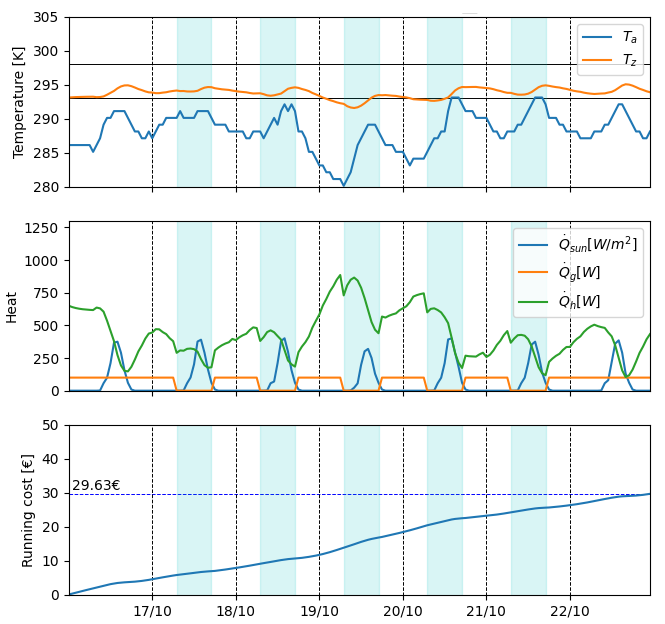
\includegraphics[scale=0.8]{images/mpc_lagrangian.png}
\caption{MPC by means of a lagrangian optimal problem for the zone heat deployment.}
\label{fig:mpc_lagrangian}
\end{figure}

\begin{figure}[H]
\centering
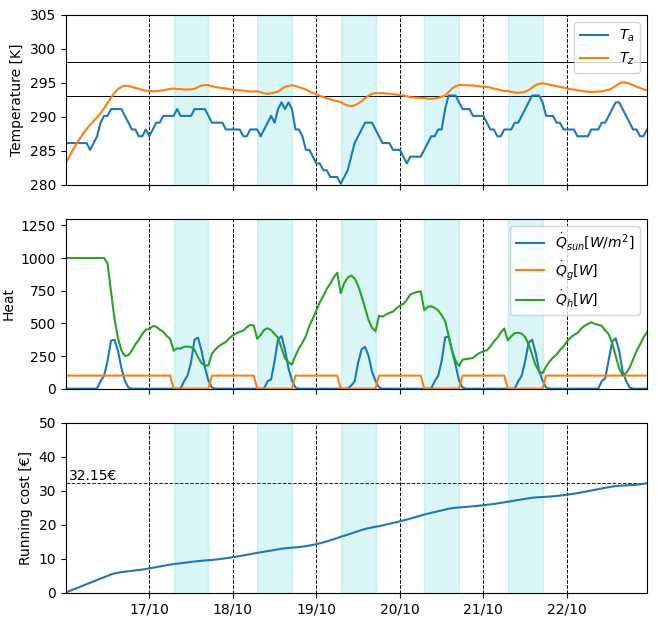
\includegraphics[scale=0.8]{images/mpc_lagrangian_Tstart.png}
\caption{MPC by means of a lagrangian optimal problem for the zone heat deployment.}
\label{fig:mpc_lagrangian_Tstart}
\end{figure}